\documentclass[a4paper,12pt]{article}
\usepackage{graphicx}
\usepackage[english]{babel}
\usepackage[T1]{fontenc}
\usepackage[utf8]{inputenc}
\usepackage{multirow}
\usepackage{amsmath}
\usepackage{float}
\usepackage{enumerate}
\usepackage{caption}
\usepackage{subcaption}
\usepackage{indentfirst}
\usepackage{color}
\usepackage{array}
\bibliographystyle{unsrt}
\usepackage[top=4cm ,bottom=4cm ,left=3cm ,right=3cm]{geometry}
\usepackage{multirow}
\usepackage{url}
\usepackage{listings}
\usepackage{color}

\definecolor{codegreen}{rgb}{0,0.6,0}
\definecolor{codegray}{rgb}{0.5,0.5,0.5}
\definecolor{codepurple}{rgb}{0.58,0,0.82}
\definecolor{backcolour}{rgb}{0.95,0.95,0.92}

\lstdefinestyle{mystyle}{
	backgroundcolor=\color{backcolour},   
	commentstyle=\color{codegreen},
	keywordstyle=\color{magenta},
	numberstyle=\tiny\color{codegray},
	stringstyle=\color{codepurple},
	basicstyle=\footnotesize,
	breakatwhitespace=false,         
	breaklines=true,                 
	captionpos=b,                    
	keepspaces=true,                 
	numbers=left,                    
	numbersep=2pt,                  
	showspaces=false,                
	showstringspaces=false,
	showtabs=false,                  
	tabsize=2
}

\lstset{style=mystyle}

\author{Alex Olar}
\title{CBM simulation}
\date{\today}

\begin{document}
\maketitle
\vfill
\begin{center}
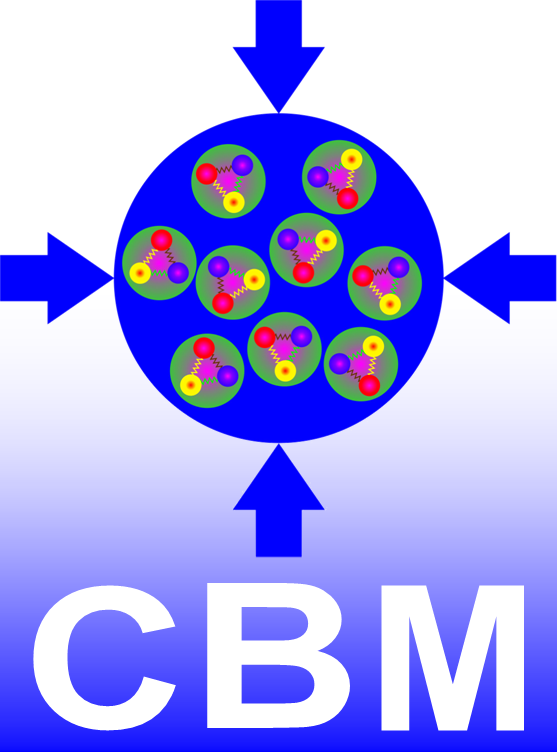
\includegraphics[width=0.66\textwidth]{gsi.png}
\end{center}
\newpage
\renewcommand{\abstractname}{Introduction}
\renewcommand{\thesection}{\Roman{section}.}
\renewcommand{\thesubsection}{\thesection\arabic{subsection}.}
\renewcommand{\thesubsubsection}{\thesubsection\arabic{subsubsection}.}
\begin{abstract}
	\par I have spent one month in summer at the GSI facility, Darmstadt to study the CBM simulation which will be part of FAIR \footnote{ Facility for Antiproton and Ion Research } . During this month I have become experienced with software such as ROOT \footnote{ CERN software for particle physics} , cbmROOT \footnote{ CBM ( Compressed Barionic Matter  ) software for heavy ion physics developped at GSI}, etc.
	\vspace{3mm}
	\par I have learned much about detector technologies and natural phenomena during my stay and I was happy to be part of this huge project and see how scientist work on a daily basis.
\end{abstract}
\tableofcontents
\newpage
\section{Fundamentals}
\subsection{QCD}
\vspace{3mm}
\par In the 20th century physicist realized that symmetries play a crucial role in further understanding the universe. Symmetries led us to conservation laws, the discovery of anti-particles, quarks and much more. 
\vspace{3mm}
\par When quarks were discovered they brought order to the ever increasing particle zoo, as Niels Bohr referred to it. At first, physicist only knew three of the six existing quarks, such as: $\textsl{u}$ (up), $\textsl{d}$ (down), $\textsl{s}$ (strange). The hadrons can be separated into two distinct groups: $\textsl{mesons}$ and $\textsl{baryons}$, containing a quark-anti-quark pair and three quarks, respectively. The property that distinguishes the quarks is called $\textsl{flavour}$.
\vspace{3mm}
\par A unique feature of the strong interaction, which is the fundamental interaction between quarks, is confinement, meaning that quarks do not appear in isolation. The charge of the strong interaction is called colours. Due to confinement it means that an elementary particle has to be colour neutral or usually referred to as ''white''. The fundamental theory describing the strong interaction is called Quantum Chromo Dynamics - QCD.
\vspace{3mm}
\par The elementary particles of the QCD are quarks and anti-quarks which interact by gluons which also carry charge. There are eight types of gluons since they must describe every elementary colour transformation. These gluons interact with themselves as well.
\subsection{ CBM physics }
\vspace{3mm}
\par When dealing with barionic matter the goal is to understand and map the phase diagram and its transitions. To begin with, I should first have to go through basic thermodynamics and its concepts about phases and their transitions.
\vspace{3mm}
\par The phase diagram of water shows the different phases of it according to pressure and temperature. It is well known that there is a triple point where all three forms of water can coexist such as: liquid water,  solid ice, and water vapor. There are distinct lines between these phases denote, along these lines two phase can coexist at the same time but when changing conditions  the substance must undergo a so called first order phase transition. There is also a critical point which is a state from where to phases differ no more, it is called a smooth $\textsl{crossover}$ from one phase to another.
\begin{figure}[H]
\centering
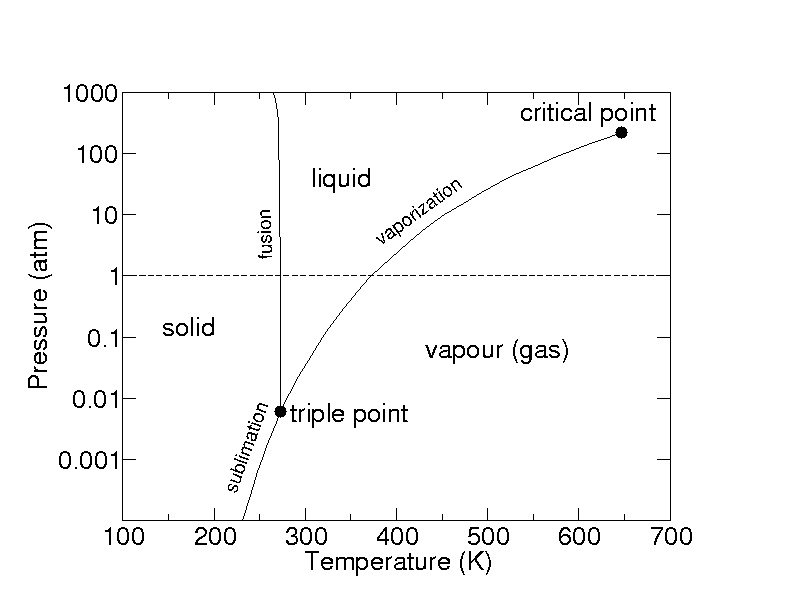
\includegraphics[width=0.66\textwidth]{water_phase.jpg}
\caption{ The previously mentioned phase diagram. }
\end{figure}
\par Now, that I went through the phase diagram of water ( or at least a part of it ) I should move on to matter governed by the strong force. The whole phase diagram of strongly interacting matter is not yet experimentally proved, purely theoretical. It depicts very different and vital phases for being able to describe the early universe or the interior of neutron stars. Each point is described by density and temperature.
 \begin{figure}[H]
\centering
\begin{subfigure}{.49\textwidth}
\centering
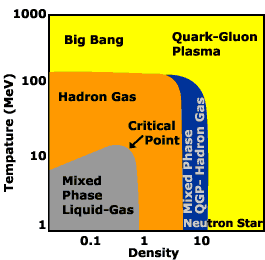
\includegraphics[width=0.92\textwidth]{cbm_phase1.png}
\caption{ Temperature in MeV and densities in units of nuclear bulk density, both scales are rhythmical }
\end{subfigure}
\begin{subfigure}{.49\textwidth}
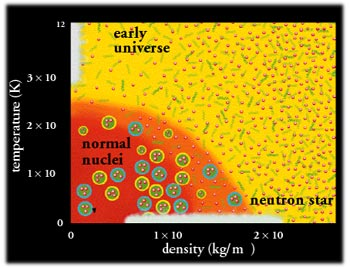
\includegraphics[width=.92\textwidth]{cbm_phase2.jpg}
\caption{ The same diagram that shows why each phase can be crucial to explore further.  }
\end{subfigure}
\end{figure}
 \par As presented above a phase called quark-gluon plasma was present at the Big Bang and later on ceased to exist when temperature dropped. It can be seen that the interior of neutron stars supposedly contains quark-gluon plasma as well as the density is high enough to enable matter to exist in that phase although the very low temperature. 
\vspace{3mm}
\par Obviously the only way to investigate strongly interacting matter on Earth is via high energy particle collisions. It is a characteristic feature of QCD that the coupling between quarks decreases as the collision energy is raised ( crossover ). This is referred to as asymptotic freedom. Another interesting symmetry of particle physics is chirality. It describes whether the particle's spin points to its direction of motion or to the opposite if the particles is massless. If the velocity and spin are pointing to the same direction the particle is called right-handed, otherwise left-handed. Due to the fact that the up and down quarks have such a small mass QCD has approximate chiral symmetry. However, this is spontaneously broken at low temperatures and densities because of the slight difference in the mass of the lightest quarks. For this reason one chiral direction is favored over the other.
\section{CBM detector}
\subsection{Theory}
\vspace{3mm}
\par The analysis of heavy nuclei collisions is extremely complex since the transient nature of the reaction. The goal is to find out more about phase diagram but the collision takes $10^{-22}~s$ and the strongly interacting matter can only be measured by the byproducts of the collision.
\par Over the past decade the main experimental activity occurred in RHIC \footnote{ Relativistic Heavy Ion Collider - Brookhaven } and at the LHC \footnote{ CERN - Large Hadron Collider }, On one hand these facilities produce important results concerning the phase diagram. These facilities are mapping the low density, high temperature area of the phase diagram and can analyze the crossover between hadron gas phase and quark-gluon plasma. On the other hand, the FAIR project is going to create much higher baryon densities to be able to explore the first-order phase transition and the critical end point of it.
\begin{figure}[H]
	\centering
	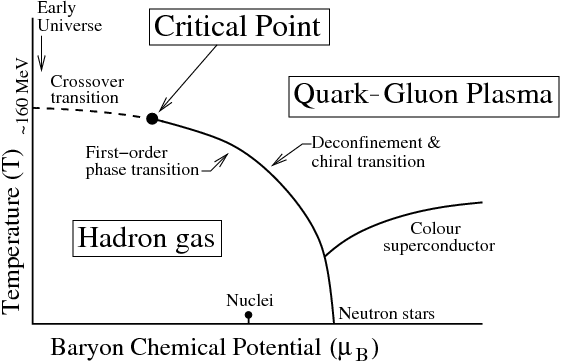
\includegraphics[width=0.40\textwidth]{CBM_phase_trans.png}
	\caption{ The above discussed hypothetical phase diagram and the transitions between phases. }
\end{figure}
\subsection{Setup and simulation}
\par The setup of the future CBM detector is the following from left to right.
\begin{itemize}
	\item CBM superconducting magnet with silicon spectrometer
	\item the micro vertex detector ( MVD ) is inside of this
	\item the silicon tracking system ( STS ) is as well
	\item ring imaging Cherenkov detector ( RICH - light blue )
	\item followed by four layers of transition radiation ( TRD ) detectors
	\item and a time-of-flight ( TOF ) wall
	\item after the main detectors there's a muon spectrometer and a projectile spectator detector ( PSD )  
\end{itemize}
\begin{figure}[H]
	\centering
	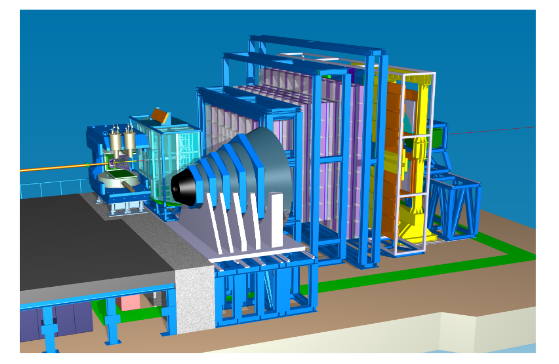
\includegraphics[width=0.66\textwidth]{cbm_detector.png}
	\caption{ View of the setup }
\end{figure}
\par The silicon tracking system is intended to reconstruct the trajectories of the particles it detects. It can only detect charged particles but also able to detect their momenta as well. The time-of-flight wall can achieve high resolution time measurements of about 60 ps.
\vspace{3mm}
\par The CBM project is currently only a plan. The construction of FAIR has started this summer and the first beams are expected by 2022. Until then CBM intends to install a reduced setup at the accelerator available at the GSI to test the systems and prepare for data processing.
\vspace{3mm}
\par Scientist of the FAIR project has developed a robust simulation so far built on ROOT. They call it cbmROOT and is available to the public. They use different well-known heavy ion collision simulation methods such as: UrQMD \footnote{ Ultra Relativistic Quantum Molecular Dynamics } or PHSD \footnote{ Parton Hadron String Dynamics }. These models are widely used among scientist in the field.
\section{My project}
\subsection{$\Phi$-meson reconstruction}
\vspace{3mm}
\par CBM is going to be a general-purpose heavy ion experiment to study the phase diagram of strongly interacting matter. Resonances are highly useful to study the high density matter created during the collisions. One of these is the $\Phi$-meson which has a small hadronic cross section so  it's  very unlikely to interact with the huge amount of hadrons. The $\Phi$-meson is made of a strange and an anti-strange quark and can be a tool to study strangeness production in the partonic phase. The $\Phi$-meson decays into $K^{+}$,$K^{-}$ pairs with an approximate of 50 \% chance and to dileptons. The mean lifetime of a $\Phi$-meson is really short, $1.55\cdot10^{-22}~s$ so it might decay into kaons and dileptons during the collision and only the byproducts would be detected by the detectors. It's mass is $1.019~MeV$ which can be seen in the invariant mass of the kaons as a peak.
\vspace{3mm}
\par I analyzed data acquired by PHSD simulation. It was an Au+Au central collision at $\sqrt{s} = 10~GeV$. The output of the simulation was passed through cbmROOT reconstruction. There were more than $5 million$ events in the $.root$ file I used for analysis.
\vspace{3mm}
\par On a histogram where the x-axis represents the invariant mass of $K^{+}$,$K^{-}$ pairs and the y-axis the entries, a clear peak can be seen on the combinatorial background at approximately $1.02~GeV$. Those were the produced $\Phi$-mesons during the collision.
\begin{figure}[H]
	\centering
	\begin{subfigure}{0.49\textwidth}
		\centering
		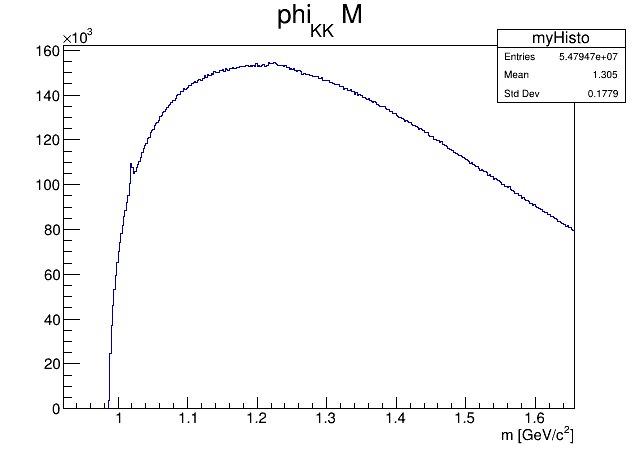
\includegraphics[width=0.95\textwidth]{phi_KK_M.png}
		\caption{ The combinatorial background and a small but recognizable peak. }
	\end{subfigure}
	\begin{subfigure}{0.49\textwidth}
		\centering
		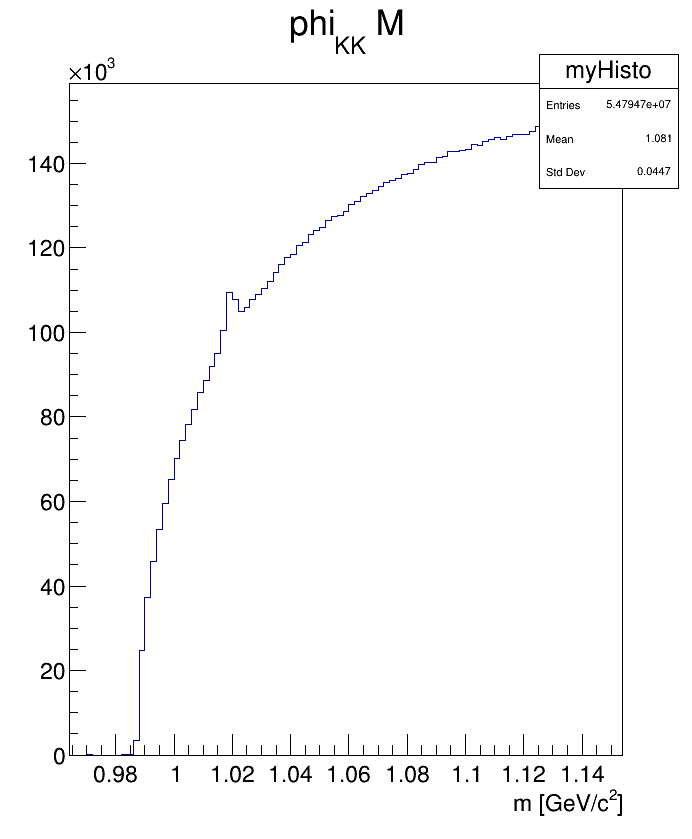
\includegraphics[width=0.95\textwidth]{phi_KK_Mzoom.png}
		\caption{ Zoomed in on the region of interest. }
	\end{subfigure}
\end{figure}
\par I tried to approximate the background with a second order polynomial. The acquired parameters for this were ($ax^{2} + bx +c$) :
\begin{center}
	\begin{tabular}{|c|c|c|}
		\hline
		Parameter name & Value [] & Error \\
		\hline
		a & -7.70559e+06 & 78750.5 \\
		\hline
		b & 1.42738e+07 & 150055 \\
		\hline
		c & -6.49147e+06 & 71438.9 \\
		\hline
	\end{tabular}
\end{center}
\par Here the fit of the background:
\begin{figure}[H]
	\centering
	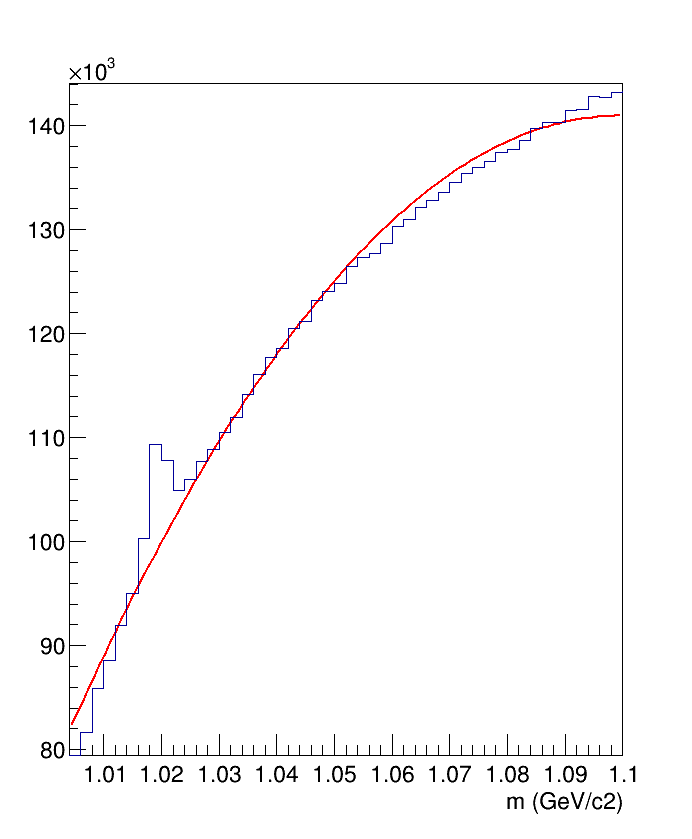
\includegraphics[width=0.35\textwidth]{combiback_fit.png}
	\caption{ The fit of the combinatorial background. }
\end{figure}
\par For the peak I used a different method. I used a low multiplicity signal to approximate the shape of the peak with a Gaussian function and then scaled that shape up to the peak with the background still remaining the same. Here are my results:
\begin{figure}[H]
	\centering
	\begin{subfigure}{0.49\textwidth}
		\centering
		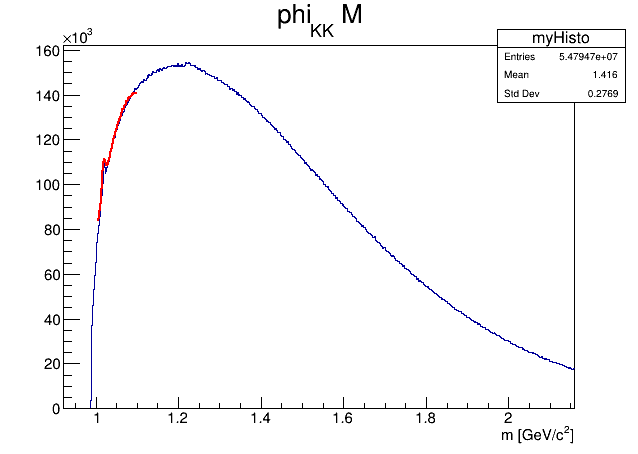
\includegraphics[width=0.95\textwidth]{phi_KK_Mfit.png}
		\caption{ The combinatorial background and a small but recognizable peak fitted. }
	\end{subfigure}
	\begin{subfigure}{0.49\textwidth}
		\centering
		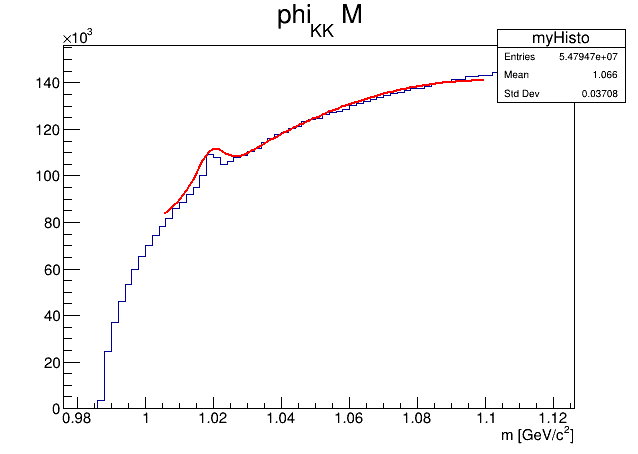
\includegraphics[width=0.95\textwidth]{phi_KK_Mfitzoom.png}
		\caption{ Zoomed in on the region of interest. }
	\end{subfigure}
\end{figure}
\par I include the ROOT macro I used for the analysis.
\lstinputlisting[language=C++]{fit.C}
\end{document}
